% -----------------------------------------------
% Template for ISMIR Papers
% 2016 version, based on previous ISMIR templates

% Requirements :
% * 6+1 page length maximum
% * 2MB maximum file size
% * Copyright note must appear in the bottom left corner of first page
% (see conference website for additional details)
% -----------------------------------------------

\documentclass{article}
\usepackage{ismir,amsmath,cite}
\usepackage{graphicx}
\usepackage{dsfont}
\usepackage{url}
\usepackage{color}

\usepackage{epstopdf} % convert eps to pdf
%\usepackage{dblfloatfix}

\usepackage{amsfonts}
\usepackage{bm}
\usepackage{stmaryrd}
\usepackage{xspace}
\usepackage{IEEEtrantools}
\newcommand*{\eg}{e.g.\@\xspace}
\newcommand*{\ie}{i.e.\@\xspace}
\newcommand*{\etal}{et al.\@\xspace}

\usepackage{amsmath}
\usepackage{graphicx}

\makeatletter
\DeclareRobustCommand{\Circ}{%
  \mathop{\vphantom{\sum}\mathpalette\Circ@\relax}\slimits@
}

\newcommand{\Circ@}[2]{%
  \vcenter{%
    \sbox\z@{$#1\sum$}%
    \hbox{\resizebox{.9\dimexpr\ht\z@+\dp\z@}{!}{$\m@th\circ$}}%
  }%
}
\makeatother

% Title.
% ------
\title{Wavelet Scattering for Automatic Chord Estimation}

% Note: Please do NOT use \thanks or a \footnote in any of the author markup

% Single address
% To use with only one author or several with the same address
% ---------------
%\oneauthor
% {Names should be omitted for double-blind reviewing}
% {Affiliations should be omitted for double-blind reviewing}

% Two addresses
% --------------
%\twoauthors
%  {First author} {School \\ Department}
%  {Second author} {Company \\ Address}

%% To make customize author list in Creative Common license, uncomment and customize the next line
%  \def\authorname{First Author, Second Author} 


% Three addresses
% --------------
\threeauthors
 {First Author} {Affiliation1 \\ {\tt author1@ismir.edu}}
  {Second Author} {\bf Retain these fake authors in\\\bf submission to preserve the formatting}
  {Third Author} {Affiliation3 \\ {\tt author3@ismir.edu}}

%% To make customize author list in Creative Common license, uncomment and customize the next line
%  \def\authorname{First Author, Second Author, Third Author} 

% Four or more addresses
% OR alternative format for large number of co-authors
% ------------
%\multauthor
%{First author$^1$ \hspace{1cm} Second author$^1$ \hspace{1cm} Third author$^2$} { \bfseries{Fourth author$^3$ \hspace{1cm} Fifth author$^2$ \hspace{1cm} Sixth author$^1$}\\
%  $^1$ Department of Computer Science, University , Country\\
%$^2$ International Laboratories, City, Country\\
%$^3$  Company, Address\\
%{\tt\small CorrespondenceAuthor@ismir.edu, PossibleOtherAuthor@ismir.edu}
%}
%\def\authorname{First author, Second author, Third author, Fourth author, Fifth author, Sixth author}


\sloppy % please retain sloppy command for improved formatting

\begin{document}

%
\maketitle
%
\begin{abstract}
State-of-the-art automatic chord recognition systems rely on multi-band chroma representations,
Gaussian Mixture Model pattern matching, and Viterbi decoding.
This paper explores the use of Haar wavelet transforms and scattering in place of multi-band
chroma. Wavelets operating across octaves encode sums and differences in chroma bins at
different scales.
We describe both the Haar wavelet transform and deep wavelet scattering and develop an
efficient algorithm for their computation. Potential benefits of wavelet representations,
including stability to octave deformations, over multi-band chroma are discussed.
Accuracy of wavelet representations used for chord recognition is analyzed over a large
vocabulary of chord qualities.
\end{abstract}

%%%%%%%%%%%%%%%%%%%%%%%%%%%%%%%%%%%%%%%%%%%%%%%%%%
\section{Introduction}\label{sec:introduction}
% TODO write less on the metrics, more on the vocabulary, more on the purpose of wavelet
Along with lyrics and melody, chord sequences provide a succinct description of tonal music.
As such, they are often written down under the form of lead sheets, for the use of
accompanists and improvisers.
Besides its original purpose in music education and transmission, the knowledge of
harmonic content has been leveraged in music information research to address higher-level
tasks, including cover song identification \cite{ellis2007identifying},
genre recognition \cite{perez2009genre}, and lyrics-to-audio alignment
\cite{mauch2012integrating}. We refer to the review of McVicar \etal
\cite{mcvicar2014automatic} for a recent state of the art.

All evaluation metrics for automatic
chord estimation share the following minimal property:
a chord label remains the same if all its components are jointly
transposed by one octave, be it upwards or downwards.
In order to comply with this requirement, the vast majority of existing
systems rely on the chroma representation, \ie a 12-dimensional vector
derived from the constant-Q spectrum by summing up all
frequency bands which share the same pitch class according to
the twelve-tone equal temperament.
However, it should be noted that the chroma representation is not
only invariant to octave transposition, but also to any permutation
of the chord factors -- an operation known in music theory
as inversion.
Although major and minor triads are unchanged by inversion,
some rarer chords, such as augmented triads and minor seventh
tetrads, are conditional upon the position of the root.

Figure 1 illustrates the importance of disambiguating inversions
when transcribing chords, which has previously been addressed by Mauch and Dixon \cite{mauch2010approximate}. The first two voicings are identical up
to octave transposition of all the chord factors, and thus have the
same chord label $\texttt{A:min7}$.
In contrast, the third voicing is labeled as \texttt{C:maj6}
in root position, although its third inversion would correspond
to the first voicing.

\begin{figure}[t]
    \begin{center}
        \setlength{\unitlength}{1cm}
        \begin{picture}(8.5,1.5)
        \put(0,-0.5){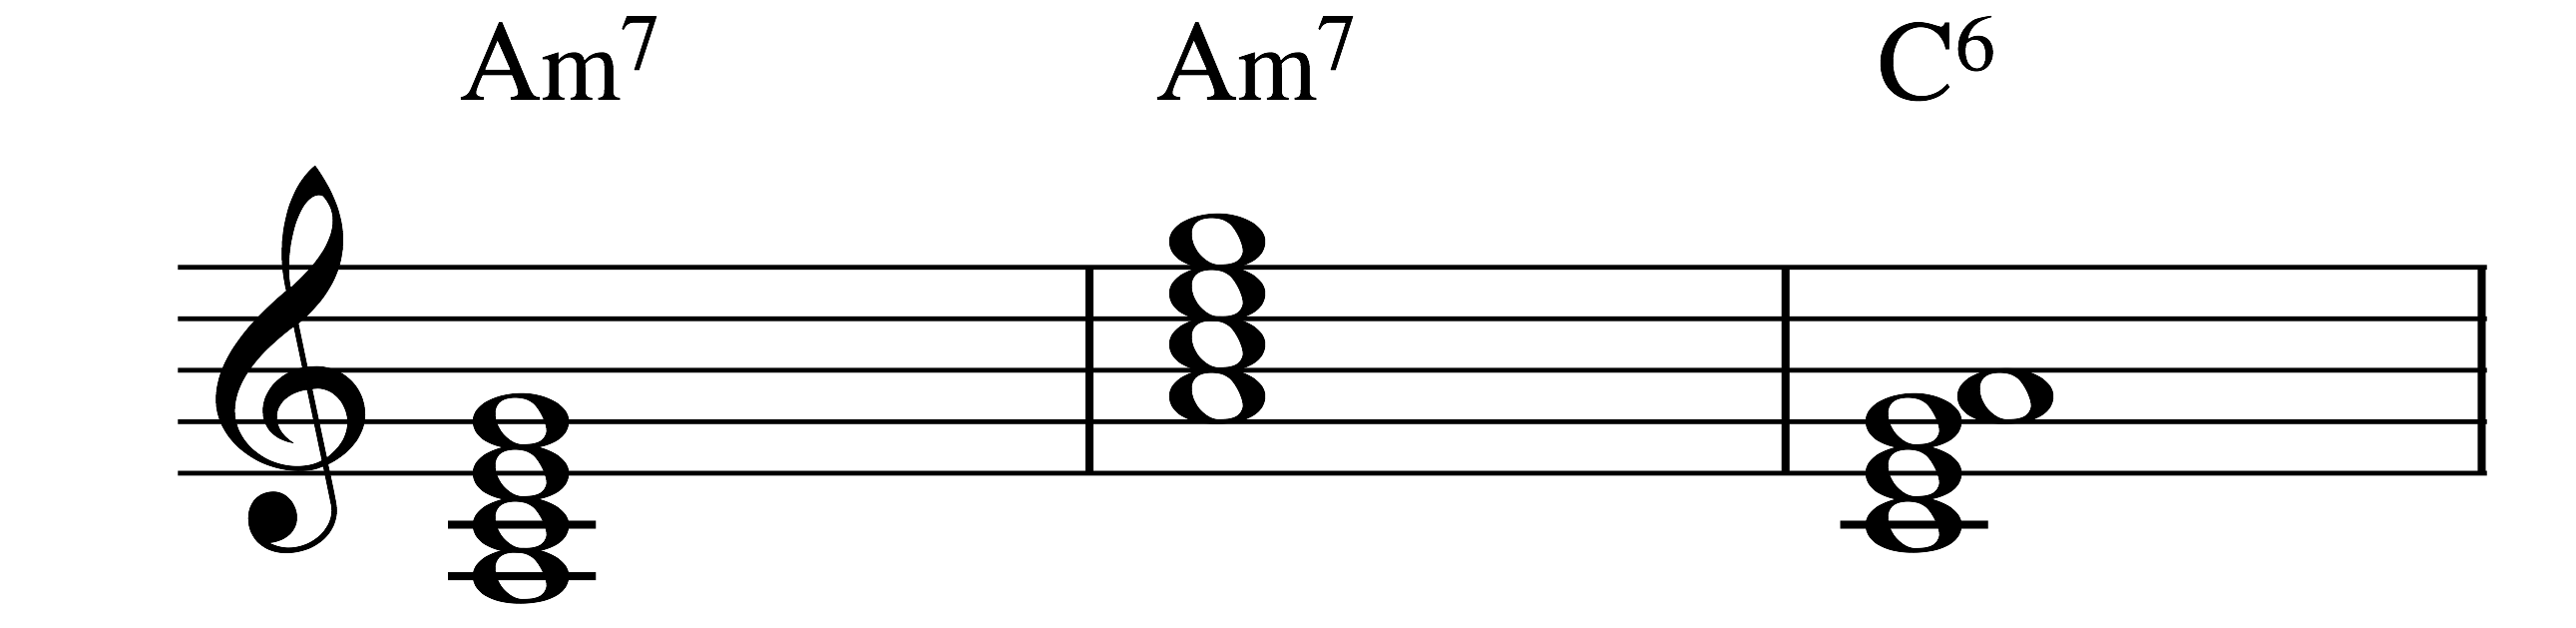
\includegraphics[width=8.5cm]{figs/sheet_music.png}}
        \end{picture}
    \end{center}
    \protect\caption{
Three possible voicings of the pitch class set
$\texttt{\{C,E,G,A\}}$, resulting either in the chord \texttt{A:min7}
or \texttt{C:maj6}. See text for details.
\label{fig:sheet-music}
}
\end{figure}

With the aim of improving automatic chord estimation (ACE) under fine-grained
evaluation metrics for large chord vocabularies (157 chord classes), this article introduces two feature extraction methods
that are invariant to octave transposition, yet sensitive to
chord inversion.
The former consists of computing a Haar wavelet transform of
the constant-Q spectrum along the octave variable and keeping
the absolute values of the resulting coefficients, at all scales
and positions.
The latter iterates the Haar wavelet modulus nonlinear operator
over increasing scales, until reaching the full extent of the
constant-Q spectrum.
Both methods build upon the large chord vocabulary ACE software of Cho and Bello
\cite{cho2013mirex}, which holds state-of-the-art performance on
the McGill Billboard dataset \cite{burgoyne2011}.

Section 2 describes the multi-band chroma features, as
introduced by Cho and Bello, and its integration into a multi-stream
hidden Markov model.
Section 3 defines the Haar wavelet transform across octaves
of the constant-Q spectrum.
Section 4 defines the deep Haar scattering transform.
Section 5 shows an example for the three representations while Section 6 presents the experimental setup along with the evaluation metrics for chord estimation accuracy. Section 7 presents the results of large vocabulary chord estimation comparing all three feature extraction methods and Section 8 discusses these results.

\section{Multi-band chroma features}
A system for automatic chord estimation typically consists of two stages:
feature extraction and acoustic modeling.
At the first stage, the audio query is converted into a time series of
pitch class profiles, which represent the relative salience of
pitch classes according to the twelve-tone equal temperament.
At the second stage, each frame in the time series is assigned
a chord label among a predefined vocabulary.
This section presents a multi-stream approach to acoustic modeling,
as first introduced by Cho and Bello \cite{cho2013mirex}.

The constant-Q transform $\mathbf{X}[t, \gamma]$ is a time-frequency
representation whose center frequencies $2^{\gamma/Q}$ are in a geometric progression.
By setting $Q=12$, the log-frequency variable $\gamma$ is akin to a pitch in twelve-tone
equal temperament.
Moreover, the Euclidean division $\gamma = Q \times u + q$
reveals the octave $u$ and pitch class $q$,
which play an essential role in music harmony.
In all of the following, we reshape the constant-Q transform
accordingly, and keep the notation $\mathbf{X}[t, q, u]$ for simplicity.

To address the disambiguation of chords in an extended vocabulary,
Cho and Bello have divided the constant-Q spectrum into $K$
bands by means of half-overlapping Gaussian windows along
the log-frequency axis \cite{cho2013mirex}.
The width $\sigma$ of the windows is inversely proportional
to the desired number of bands $K$:
in particular, it is of the order of one octave for $K=8$,
and two octaves for $K=4$.
The centers of the windows are denoted by $\gamma_k$, where
the band index $k$ ranges from $0$ to $K-1$.
Consequently, the multi-band chroma features are defined as the following
three-way tensor:
\begin{equation}
\mathbf{Y}[t, q, k]
=
\sum_{u} 
\mathbf{X}[t, q, u]
\boldsymbol{w}[Q \times u + q - \gamma_k],
\end{equation}
where
$\boldsymbol{w}[\gamma] = \exp( - \gamma^2 / (2\sigma^2))$
is a Gaussian window of width $\sigma$, centered around zero.

Acoustic modeling is classically achieved with a hidden Markov model (HMM)
whose states are estimated as mixtures of multivariate Gaussian probability
distributions, \ie Gaussian mixture models (GMM) in dimension $Q=12$.
In order to extend this framework to multi-band chroma features, Cho and Bello
have trained $K$ end-to-end models in parallel over each feature map $k$
of the tensor $\mathbf{Y}[t, q, k]$.
At test time, the emission probability distributions of each model
are aggregated such that they are the predicted outputs of a single state sequence.

The computational complexity of resulting $K$-stream HMM grows exponentially
with the number of streams $K$.
However, by assuming synchronicity and statistical independence of the streams,
the aggregation boils down to a geometric mean, thus with linear complexity in $K$.
It must be noted that the geometric mean does not yield a true probability distribution, as
it does not sum to one.
Yet, it is of widespread use \eg in speech recognition, due to its simplicity and computational
tractability.

Fed with multiband chroma features, the $K$-stream HMM
has achieved state-of-the-art results on the McGill Billboard dataset at the
MIREX evaluation campaign \cite{cho2013mirex}.

%%%%%%%%%%%%%%%%%%%%%%%%%%%%%%%%%%%%%%%%%%%%%%%%%%
\section{Haar Wavelet Transform}\label{sec:haar}
\begin{figure}[t]
    \begin{center}
        \setlength{\unitlength}{1cm}
        \begin{picture}(8.5,7)
        \put(0,-0.5){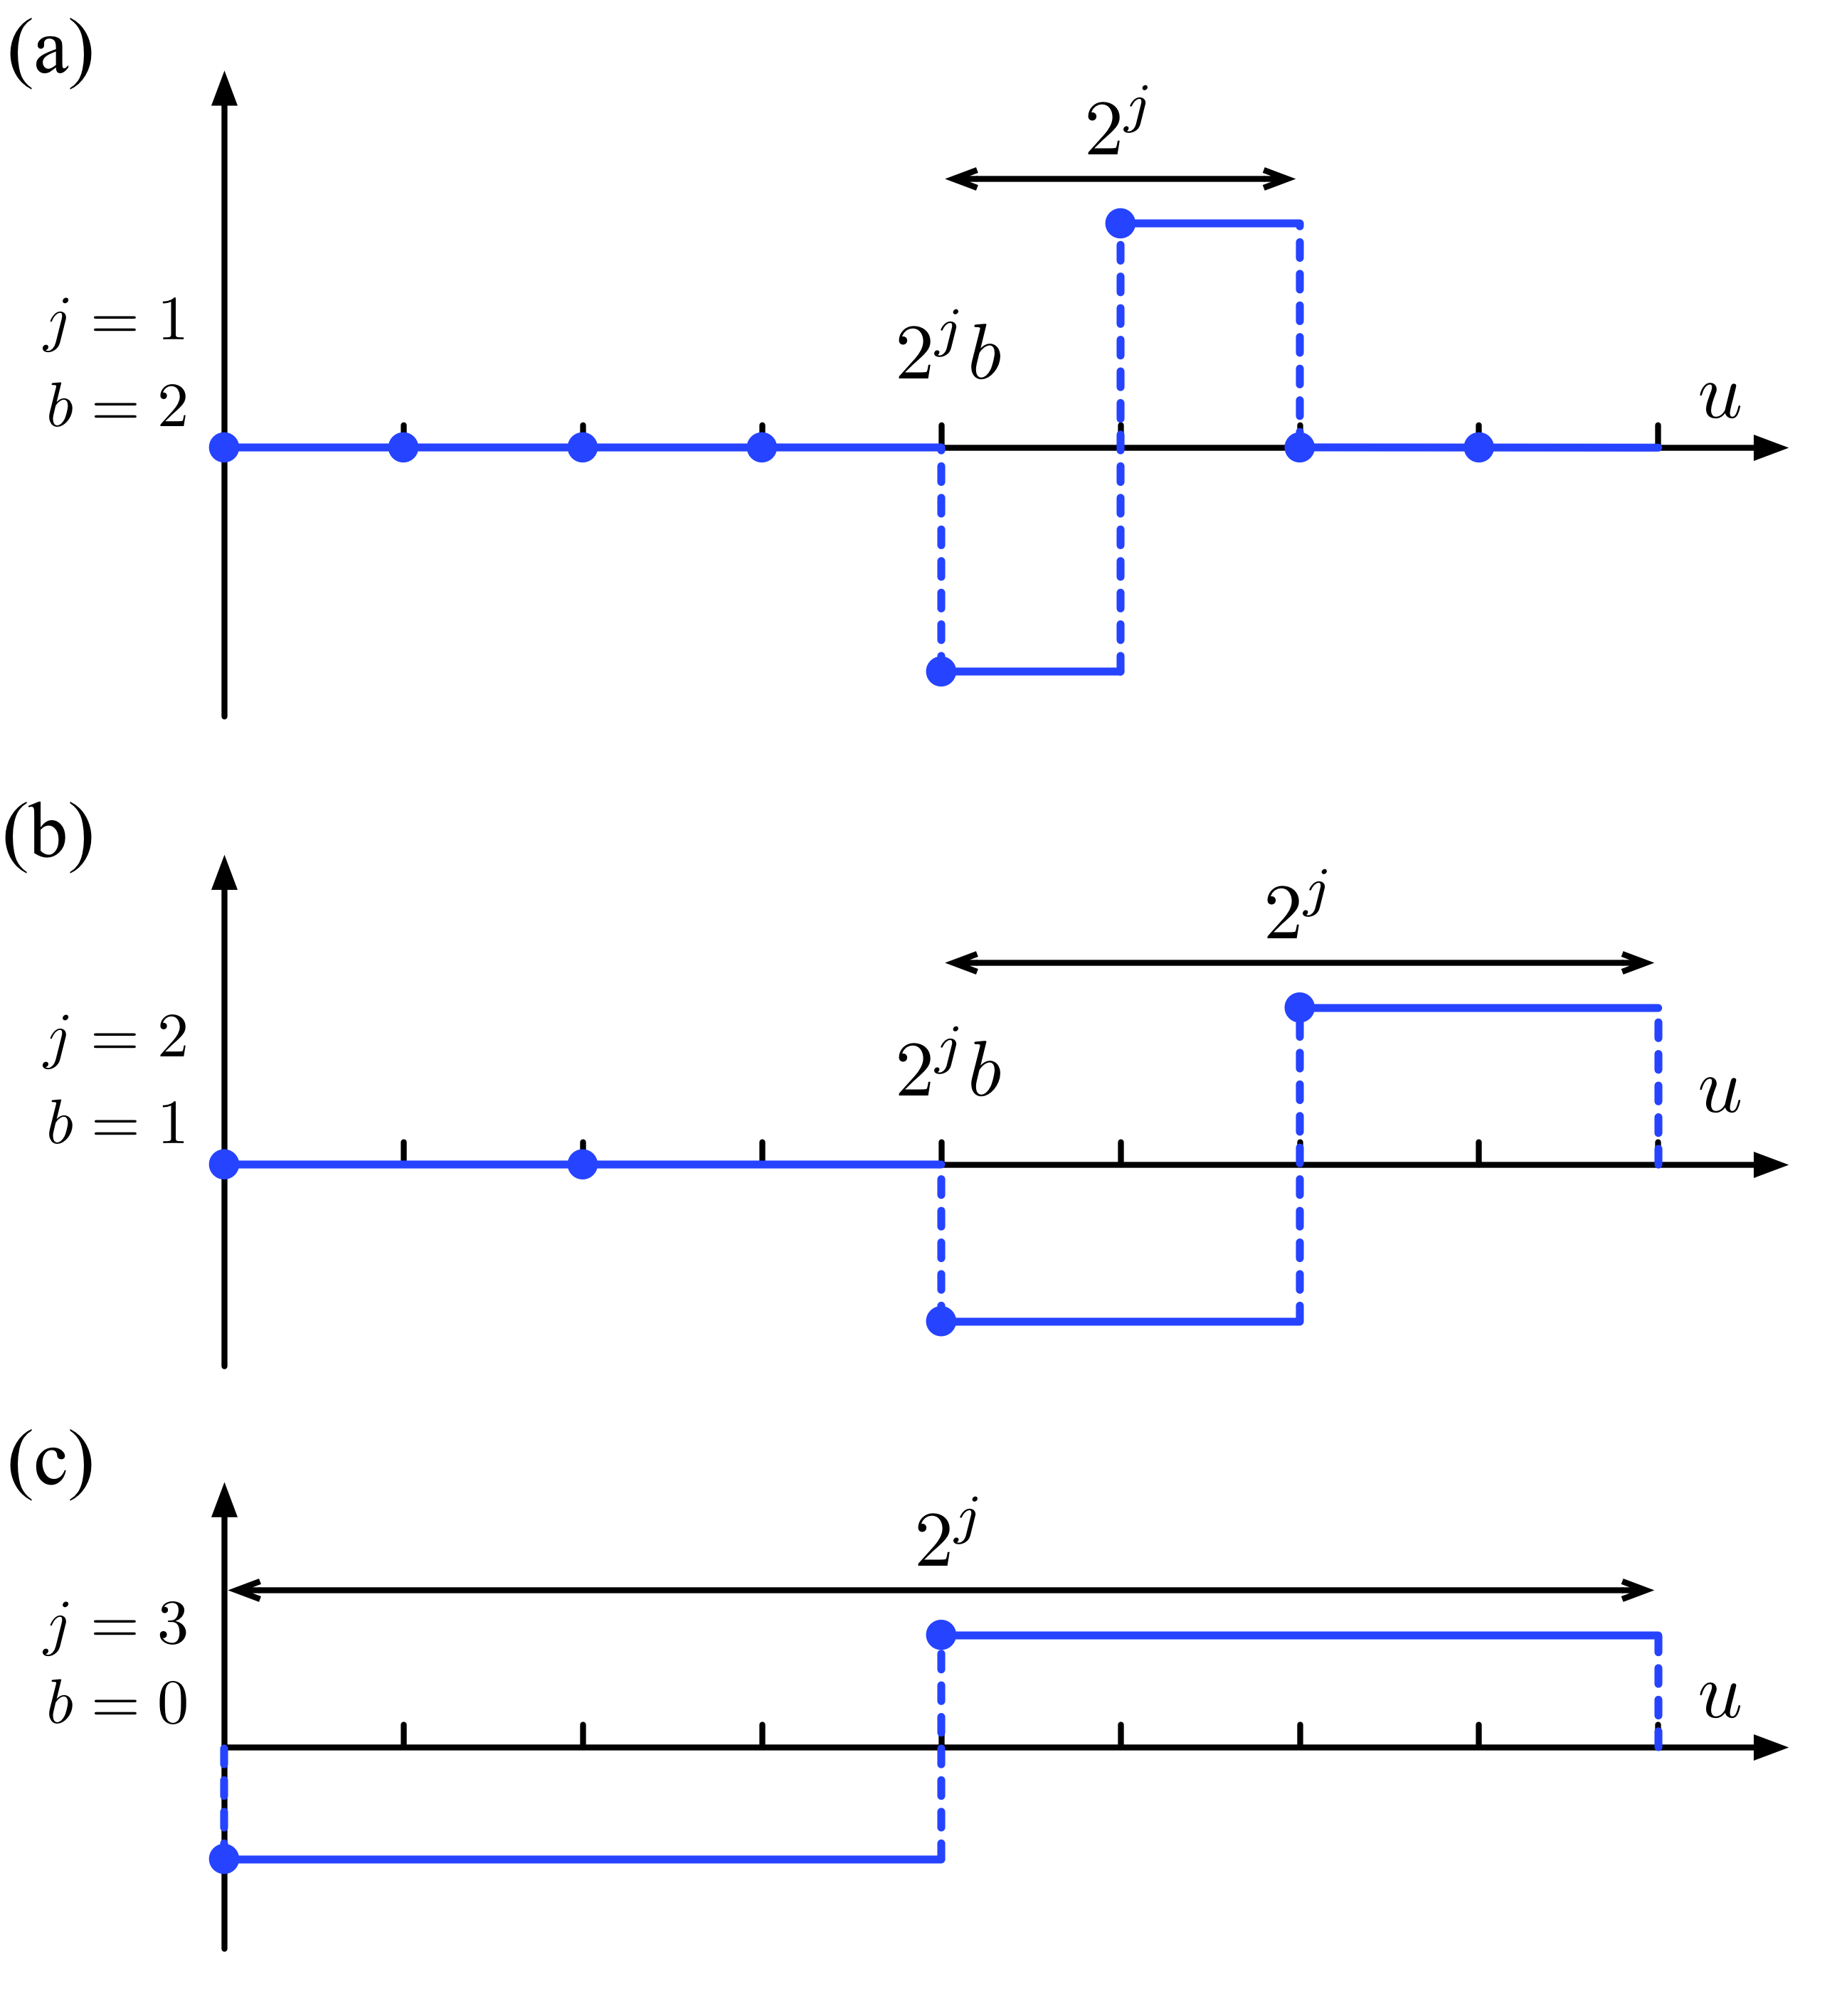
\includegraphics[width=7cm]{figs/haar_functions.png}}
        \end{picture}
    \end{center}
    \protect\caption{
Three elements of the Haar wavelet basis $\{ \boldsymbol{\psi_{j,b}}\}$
for various values of the scale index $j$ and the translation index $b$.
See text for details.
\label{fig:haar-wavelets}
}
\end{figure}
In spite of their success, the multi-band chroma features presented above are rather
unsatisfying as inputs of a $K$-stream HMM, which relies on statistical independence.
In this section, we introduce an alternative set of features for harmonic content, namely
the absolute value of Haar wavelet coefficients, which satisfies statistical independence since
it is derived from an orthogonal basis of $\mathbb{R}^K$.
All subsequent operations apply to the octave variable $u$,
and are vectorized in terms of time $t$ and chroma $q$.
To alleviate notations, we replace the three-way tensor $\mathbf{X}[t, q, u]$
by a vector $\boldsymbol{x}[u]$, thus leaving the indices $t$ and $q$ implicit.

The Haar wavelet $\boldsymbol{\psi}$ is a piecewise constant,
real function of compact support,
consisting of two steps of equal length and opposite values.
Within a discrete framework,
it is defined by the following formula:
\begin{equation}
\forall u \in \mathbb{Z}, \;
\boldsymbol{\psi}[u] = \left\{ \begin{array}{cl}
\frac{-1}{\sqrt{2}} & \mbox{if }u = 0\\
\frac{1}{\sqrt{2}} & \mbox{if }u = 1\\
0 & \mbox{otherwise}
\end{array}\right.
\end{equation}
The "mother" wavelet $\boldsymbol{\psi}[u]$ is translated and dilated by powers of two, so as to
produce a family of discrete sequences
$\boldsymbol{\psi_{j,b}}[u] = 2^{\frac{j-1}{2}} \boldsymbol{\psi}[2^{(j-1)} (u - 2b)]$
indexed by the scale parameter $j \in \mathbb{N^*}$
and the translation parameter $b \in \mathbb{Z}$.
Some Haar wavelets are shown on Figure \ref{fig:haar-wavelets}
for various values of $j$ and $b$.
After endowing them with the Euclidean inner product
\begin{equation}
\langle \boldsymbol{\psi_{j,b}} \vert \boldsymbol{\psi_{j^\prime,b^\prime}} \rangle
 =
 \sum_{u = -\infty}^{+\infty}
 \boldsymbol{\psi_{j, b}}[u]
  \boldsymbol{\psi_{j^\prime,b^\prime}}[u],
\end{equation}
the wavelets $\{\boldsymbol{\psi_{j,b}}\}_{j,b}$ form an orthonormal basis of finite-energy
real sequences.
Moreover, the Haar wavelet is the shortest function of compact support such that the family
$\{\boldsymbol{\psi_{j,b}}\}_{j,b}$ satisfies this orthonormality property.
On the flip side, it has a poor localization in the Fourier domain, owing to its sharp discontinuities.

It must be noted that, unlike the pseudo-continuous variables of time and frequency,
the octave variable is intrinsically dicrete, and has no more than 8 coefficients in
the audible spectrum.
Therefore, we choose to favor compact support over regularity, \ie Haar over
Daubechies or Gabor wavelets.

The wavelet transform of some finite-energy sequence
$\boldsymbol{x} \in \ell^2(\mathbb{Z})$ is defined by
$\mathbf{W} \boldsymbol{x}[j, b]
= \langle \boldsymbol{x} \vert \boldsymbol{\psi_{j,b}} \rangle$.
Since $\boldsymbol{x}[u]$ has a finite length $K = 2^J$,
this decomposition is informative only for indices $(j, b)$
such that $j \leq J$ and $2^j b \leq K$, \ie $b\leq2^{J-j}$.
The number of coefficients in the Haar wavelet transform of $\boldsymbol{x}[u]$ is thus equal to
$\sum_{j =1}^{J} 2^{J-j} = 2^J - 1$. For the wavelet representation to
preserve energy and allow signal reconstruction, a residual term
\begin{equation}
\boldsymbol{\mathbf{A}_J} \boldsymbol{x}
= \boldsymbol{x}[0] -
\sum_{j,b}
\langle \boldsymbol{x} \vert \boldsymbol{\psi_{j,b}} \rangle \boldsymbol{\psi_{j,b}}[0]
= \sum_{u<K} \boldsymbol{x}[u]
\label{eq:lowpass-term}
\end{equation}
must be appended to the wavelet coefficients.
Observe that $\boldsymbol{\mathbf{A}_J}  \boldsymbol{x}$
computes a delocalized average of all signal coefficients,
which can equivalently be formulated as an inner product with the constant
function $\boldsymbol{\phi}[u] = 2^{-J/2}$ over the support $\llbracket 0 ; K \llbracket$.
Henceforth, it corresponds to the traditional chroma representation, where spectrogram bands
of the same pitch class $q$ are summed across all $K$ octaves.

Since the wavelet representation amounts to $K$ inner products in $\mathbb{R}^K$,
its computational complexity is $\Theta(K^2)$ if implemented as a matrix-vector product.
Fast Fourier Transforms (FFT) would bring the complexity to
$\Theta{(K (\log_2 K)^2)}$.
To improve this, Mallat has developed a recursive scheme, called
\emph{multiresolution pyramid} \cite{mallat1989theory}, which operates as a cascade
of convolutions with some pair of quadrature mirror filters
$(\boldsymbol{g}, \boldsymbol{h})$ and progressive subsamplings by a factor of two.
Since the number of operations is halved after each subsampling, the total
complexity of the multiresolution pyramid is $K + \frac{K}{2} + \cdots + 1 = \Theta(K)$.

Let us denote by $\boldsymbol{g}_{\downarrow 2}$ and
$\boldsymbol{h}_{\downarrow 2}$ the corresponding operators of subsampled
convolutions, and by $(\boldsymbol{g_{\downarrow 2}})^j$ the $j$-fold composition
of operators $\boldsymbol{g_{\downarrow 2}}$.
The wavelet transform rewrites as
\begin{equation}
\mathbf{W}\boldsymbol{x}[j,b] =
\left(
\boldsymbol{h_{\downarrow 2}} \circ
(\boldsymbol{g_{\downarrow 2}})^j \boldsymbol{x}
\right)[b],
\end{equation}
while the fully delocalized chroma representation rewrites as
$\boldsymbol{\mathbf{A}_J} \boldsymbol{x} =
(\boldsymbol{g_{\downarrow 2}})^J \boldsymbol{x}$.
A flowchart of the operations involved in the wavelet transform is shown on
Figure \ref{fig:wavelet-flowchart}.
We refer to chapter 7 of \cite{mallat2008wavelet}
for further insight.

\begin{figure}[t]
    \begin{center}
        \setlength{\unitlength}{1cm}
        \begin{picture}(8,2.5)
        \put(0,-0.5){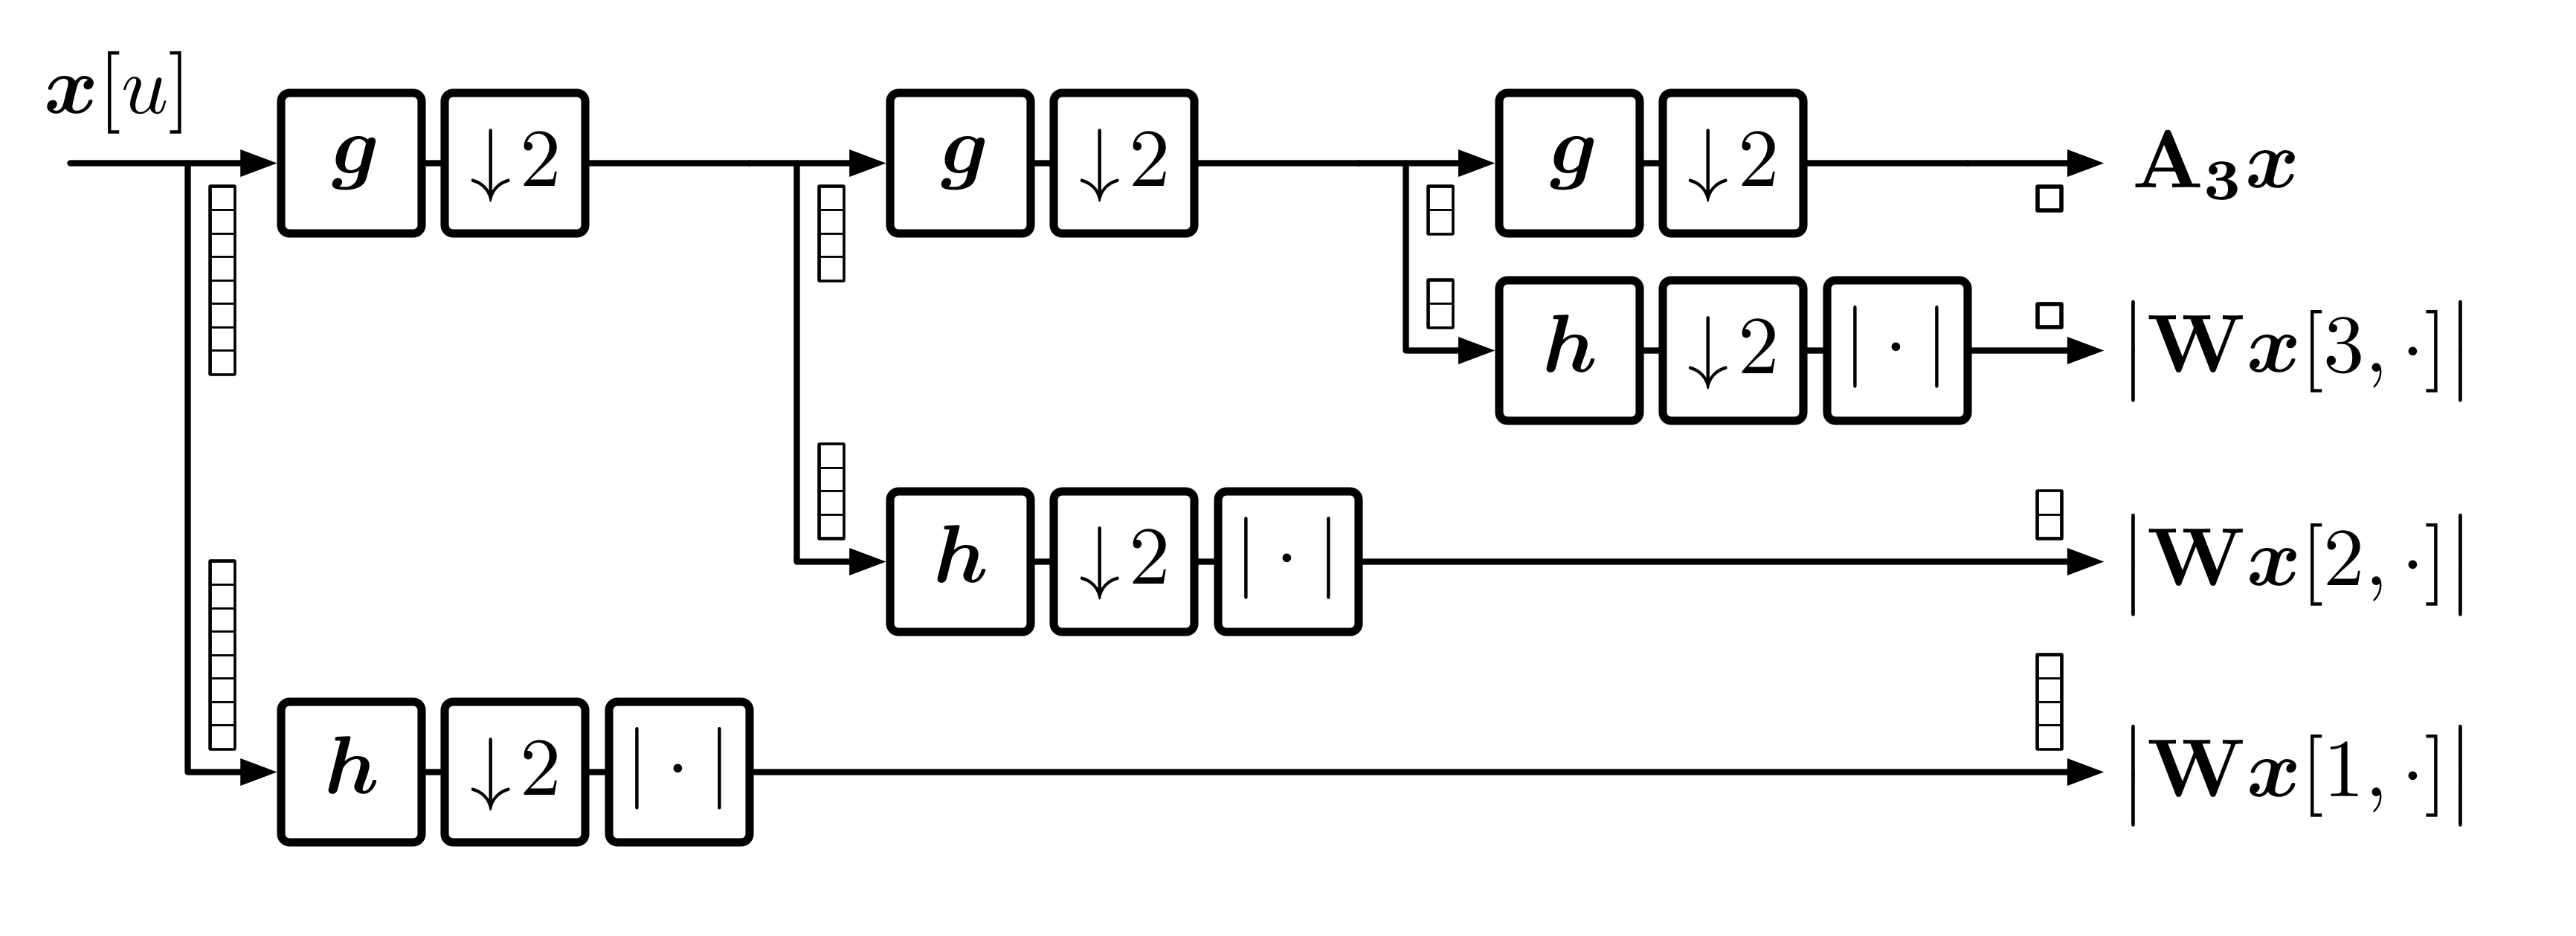
\includegraphics[width=8.2cm]{figs/wavelet_scheme.png}}
        \end{picture}
    \end{center}
    \protect\caption{
    Discrete wavelet transform of a signal of length $K=8$, as implemented with a
    multiresolution pyramid scheme. See text for details.
\label{fig:wavelet-flowchart}
}
\end{figure}
Since the low-pass filter $\boldsymbol{\phi}$ and the family of
wavelets $\boldsymbol{\psi_{j,b}}$'s form an orthonormal basis of $\mathbb{R}^K$,
any two signals $\boldsymbol{x}[u]$ and $\boldsymbol{y}[u]$ have the same
Euclidean distance in the wavelet domain as in the signal domain.
This isometry property implies that the wavelet representation is not
invariant to translation per se.
Therefore, the wavelet-based chroma features are extracted by taking
the absolute value of each wavelet coefficient, hence contracting
Euclidean distances in the wavelet domain.
Most importantly,
the distance $\Vert \mathbf{W}\boldsymbol{x} - \mathbf{W}\boldsymbol{y} \Vert$
is all the more reduced by the absolute value nonlinearity
that $\boldsymbol{x}$ and $\boldsymbol{y}$ are approximate
translates of each other.

In the case of Haar wavelets, the low-pass filtering $(\boldsymbol{x} \ast \boldsymbol{g})$
consists of the sum between adjacent coefficients, whereas the high-pass filtering
$(\boldsymbol{x} \ast \boldsymbol{h})$ is the corresponding difference, up to a
renormalization constant:
\begin{IEEEeqnarray}{rCl}
(\boldsymbol{x} \ast \boldsymbol{g})[2b]
& = &
\frac{ \boldsymbol{x}[2b+1] + \boldsymbol{x}[2b]}{\sqrt{2}}$, and$
\nonumber \\
(\boldsymbol{x} \ast \boldsymbol{h})[2b]
&= &
\frac{ \boldsymbol{x}[2b+1] - \boldsymbol{x}[2b]}{\sqrt{2}}.
\IEEEeqnarraynumspace
\end{IEEEeqnarray}

Besides its small computational complexity, the multiresolution pyramid
scheme has the advantage of being achievable without allocating memory.
Indeed, at every scale $j$, the pair
$(\boldsymbol{g_{\downarrow 2}}, \boldsymbol{h_{\downarrow 2}})$
has $2^{-j} K$ inputs and $2^{-j} K$ outputs, of which one half are
subsequently mutated.
By performing the sums and differences in place, and deferring the
renormalization to the end of the flowchart, the time taken by the
wavelet transform procedure remains negligible in front
of the time taken by the constant-Q transform.

%\begin{table}
%	\begin{center}
%	\begin{tabular}{|c|cc|}
%		\hline
%		& operations & memory \\
%		\hline
%		Matrix-vector product & $\Theta(K^2)$ & $\Theta(K)$ \\
%		Fast Fourier transforms & $\Theta(K (\log K)^2)$ & $\Theta(K)$ \\
%		Multiresolution pyramid & $\Theta(K)$ & $\Theta(1)$ \\
%		\hline		
%	\end{tabular}
%	\end{center}
%	\caption{
%	Computational complexity and memory usage of various implementations
%	of the Haar wavelet transform, for a one-dimensional signal of length $K$.
%	See text for details.
%	\label{table:wavelet-complexities}}
%\end{table}


%%%%%%%%%%%%%%%%%%%%%%%%%%%%%%%%%%%%%%%%%%%%%%%%%%
\section{Deep Haar Scattering}\label{sec:scattering}
The wavelet modulus operator decomposes the variations of a signal at
different scales $2^j$ while keeping the finest localization possible $b$.
As such, the coefficient $\vert \mathbf{W} \boldsymbol{x}[j, b] \vert$
only bears a limited amount of invariance, which is of the order
of $2^j$.
In this section, we iterate the scattering operator over increasing scales,
until reaching some maximal scale $K=2^J$.
We interpret the scattering cascade in terms of invariance and discriminability,
and provide a fast implementation with $\Theta(K \log K)$ operations
and $\Theta(1)$ allocated memory.

Most of the intervallic content of chords in tonal music consists of perfect fifths,
perfect fourths, major thirds and minor thirds.
Quite strikingly, these intervals are also naturally present in harmonic series,
as the log-frequency distances between the first partials.
By combining the two previous propositions, we deduce that
the components of a typical chord overlap at high frequencies,
hence producing an interference pattern which reveals their relative positions.

In our introductory example, denoting by $f_0$ the root frequency of \texttt{A:min7},
$f_0$ interferes with its perfect fifth $\texttt{E}$ at the frequency $3 f_0$.
In contrast, in its third inversion labeled as $\texttt{C:6}$, the interference
between $\texttt{A}$ and $\texttt{E}$ only starts at $6 f_0$, \ie one octave higher.
Under the same instrumentation, this inversion yields a deformation of the
octave vector corresponding to $\texttt{E}$, which consists of the frequency bins
of the form $2^u \times 3 f_0$ for integer $u \in \mathbb{Z}$.
More generally, we argue that the characterization of complex interference patterns
in polyphonic music is a major challenge in large-vocabulary chord estimation,
as it provides a tool for disambiguating chord inversions in spite of global
invariance to octave transposition.

In this regard, the wavelet modulus operator is neither fully invariant to
octave transposition, nor does it retrieve the structure of musical chords beyond
binary interactions between overlapping partials.
Nonetheless, both of these desired properties can be progressively improved
by cascading the wavelet modulus operator over increasing scales, until
reaching the full support $2^J$ of the original signal $\boldsymbol{x}[u]$ ;
a nonlinear decomposition known as the scattering transform \cite{mallat2012group}.

Considering that Haar wavelet is analogous to a linear interferometer,
the scattering transform is a recursive interferometric representation,
whose recursion depth $m$ varies according to the number of
modulus nonlinearities encountered before reaching the scale $2^J$.
Whereas wavelet coefficients $\boldsymbol{Wx}[j,b]$ are indexed by a scale
parameter $j$ and a translation parameter $b$, scattering coefficients are
indexed by sequences of scale parameters $(j_1 \ldots j_m)$ called
\emph{paths}, and do not need a translation parameter since they are
fully delocalized.
The increasing scales in a scattering path correspond to the cumulative
sum of integers $j_1$ to $j_m$.
Therefore, the full sum $\sum_{n=1}^{m} j_n$ should be lower or equal to $J$.
If it is strictly lower than $J$, a low-pass filtering with $\boldsymbol{\phi}$ is
performed after the final wavelet modulus layer.

Scattering has been employed as a feature extraction stage for many problems in
signal classification.
Initially defined as operating solely over the time dimension, it has recently been
generalized to multi-variable transforms in the time-frequency domain,
including log-frequency and octave \cite{lostanlen2015wavelet}.
In addition, Cheng \etal have applied Haar scattering to
the unsupervised learning of unknown graph connectivities \cite{cheng2014deep}.

\begin{figure}[t]
    \begin{center}
        \setlength{\unitlength}{1cm}
        \begin{picture}(8,5)
        \put(0.1,0){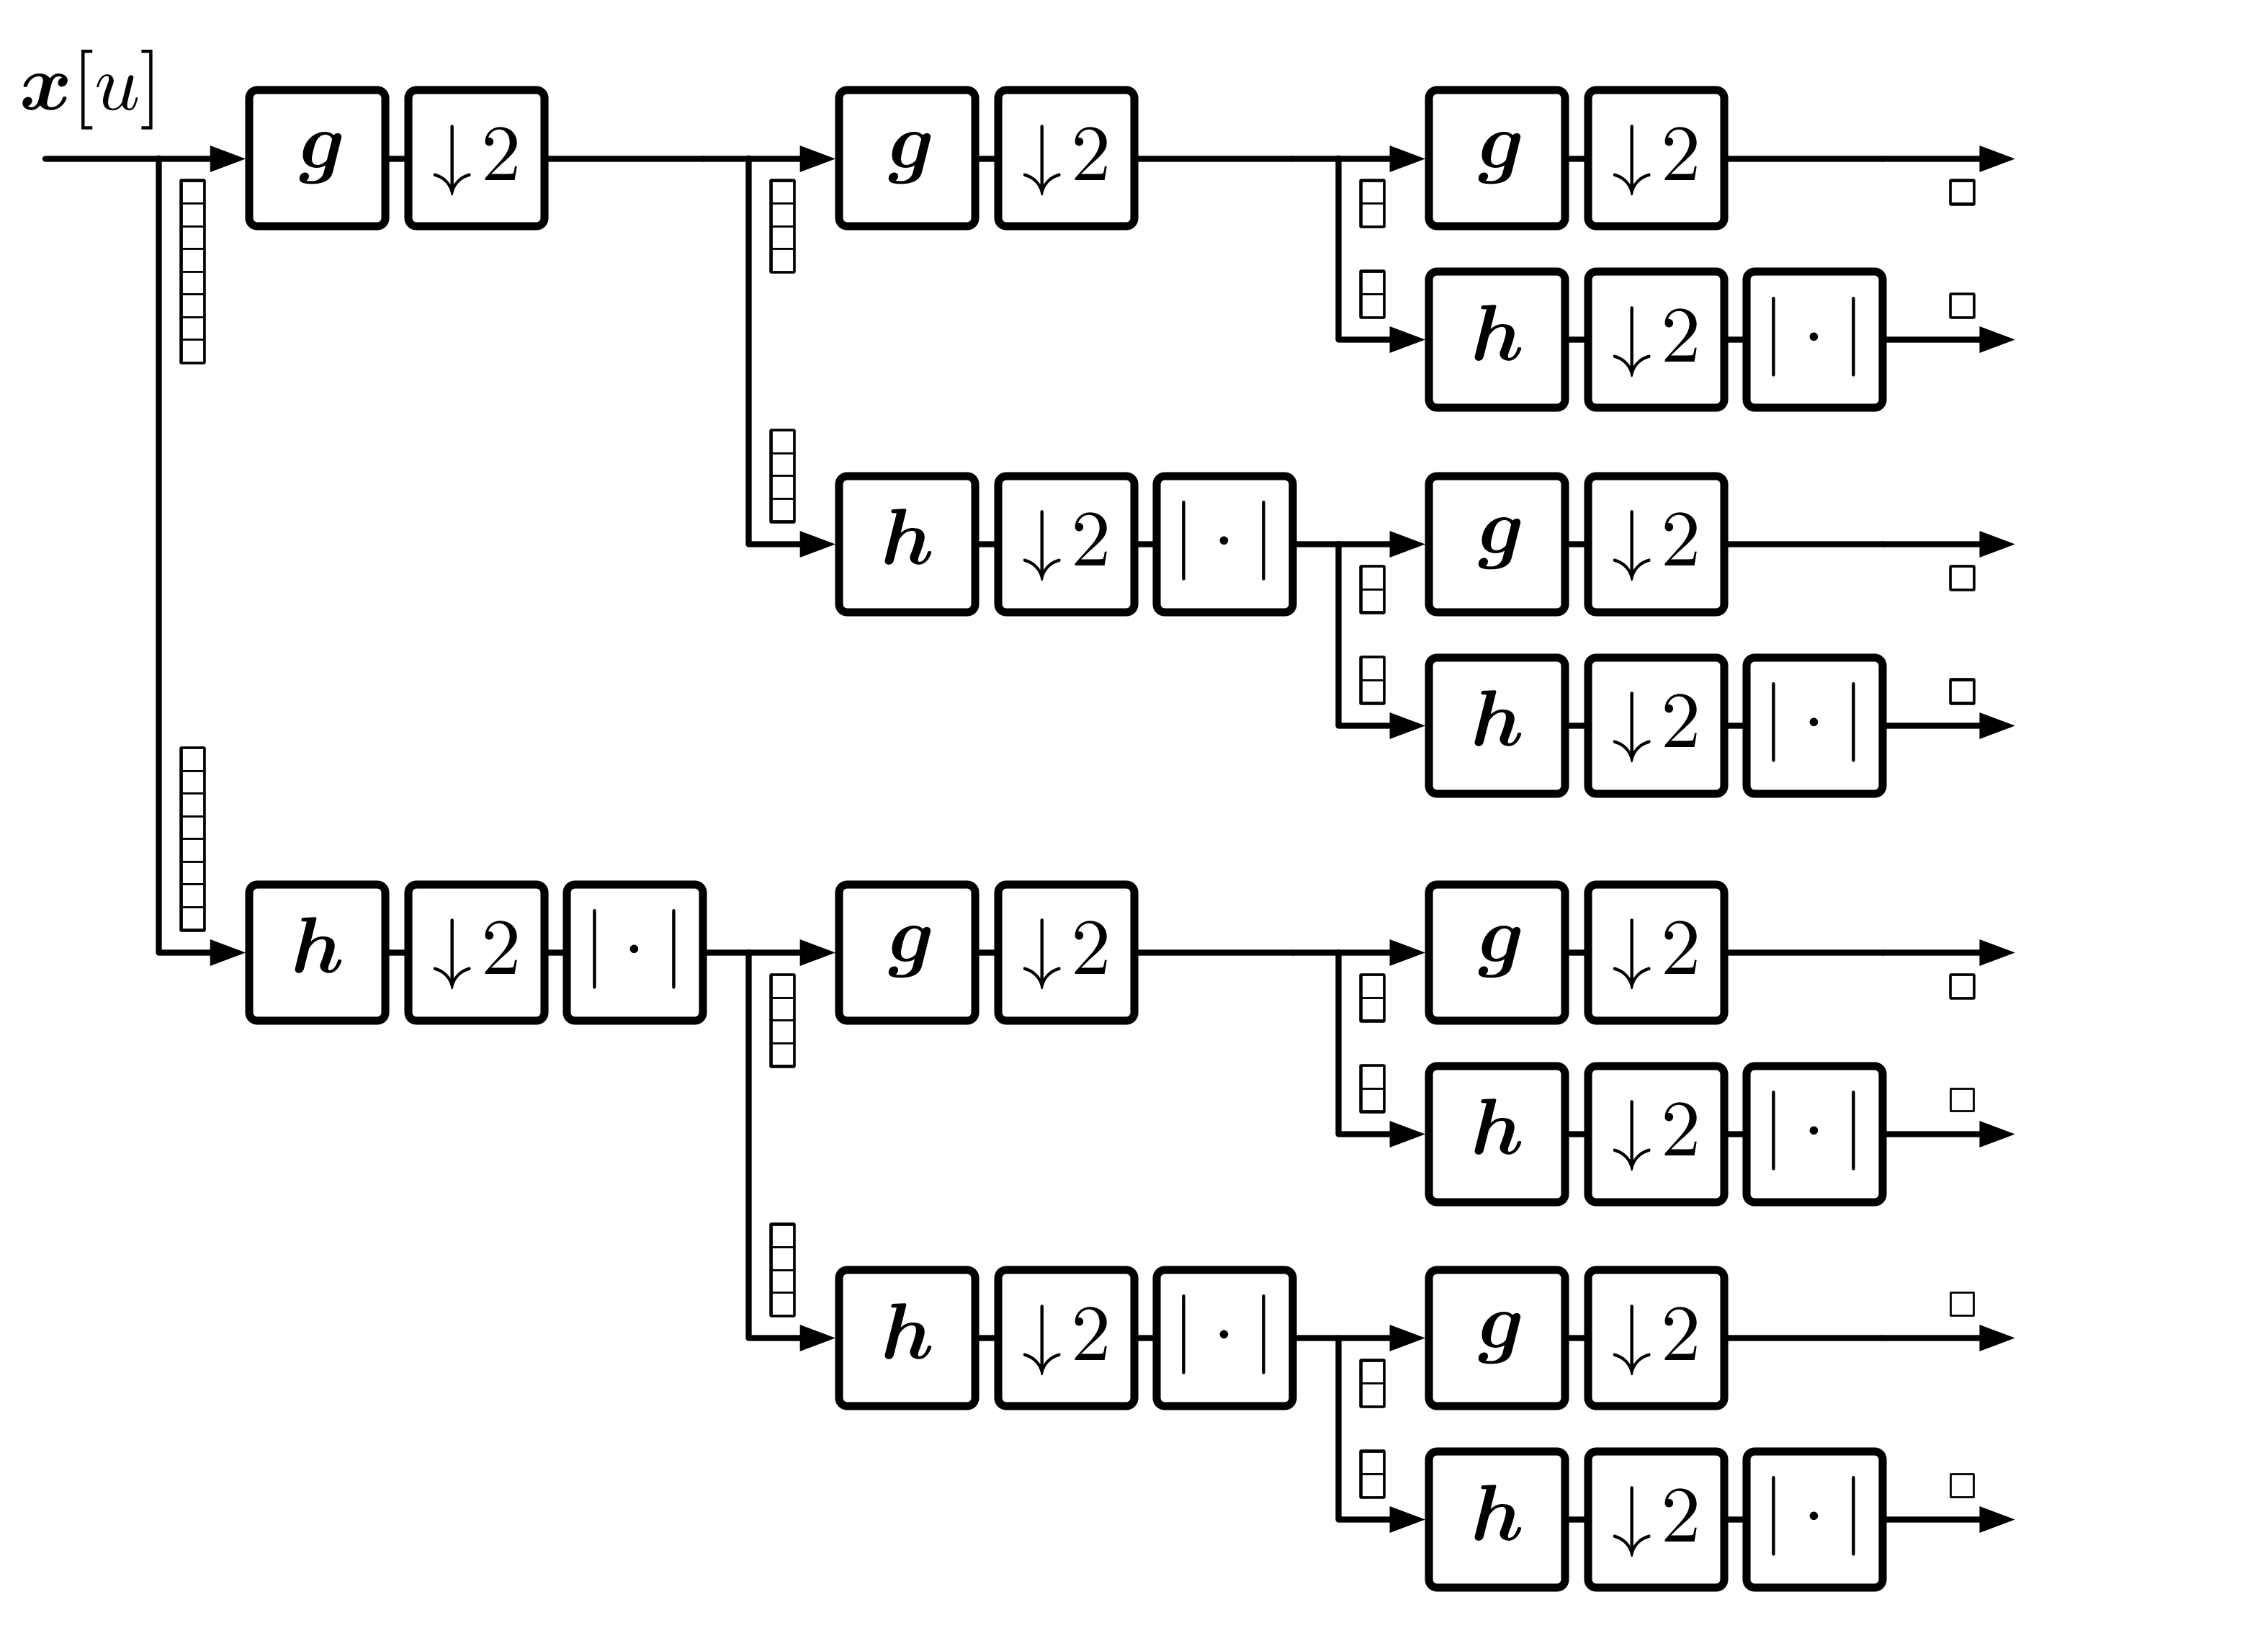
\includegraphics[width=8cm]{figs/scattering_scheme.png}}
        \end{picture}
    \end{center}
    \protect\caption{
    Deep scattering transform of a signal of length $K=8$,
    as implemented with a convolutional
    pyramid scheme. See text for details.
\label{fig:haar-scattering}
}
\end{figure}

%\begin{table}[t]
%	\begin{center}
%	\begin{tabular}{|c|cc|}
%		\hline
%		& operations & memory \\
%		\hline
%		Matrix-vector product & $\Theta(K^3)$ & $\Theta(K^2)$ \\
%		Fast Fourier transforms & $\Theta(K^2 (\log K)^2)$ & $\Theta(K^2)$ \\
%		Multiresolution pyramid & $\Theta(K \log K)$ & $\Theta(1)$ \\
%		\hline		
%	\end{tabular}
%	\end{center}
%	\protect\caption{Computational complexity and memory usage of various implementations
%	of the deep Haar scattering transform, for a one-dimensional signal
%	of length $K$. See text for details.
%	\label{table:scattering-complexities}}
%\end{table}

Since it results from the alternate composition of unitary and contractive operators,
it follows immediately that the scattering transform is itself unitary and contractive.
Moreover, Mallat has proven that it is invariant to translation and stable to the
action of small deformations \cite{mallat2012group}.
Along the octave variable $u$, translation
corresponds to octave transposition, while small deformations correspond to
variations in spectral envelope, such as those induced by a change in
instrumentation or by polyphonic interference.

Like the orthogonal wavelet transform, the scattering transform benefits
from a multiresolution pyramid recursive scheme.
By decomposing $\boldsymbol{x}[u]$ with subsampled quadrature mirror filters 
$\boldsymbol{g_{\downarrow 2}}[u]$ (low-pass) and
$\boldsymbol{h_{\downarrow 2}}[u]$ (high-pass)
over a full binary tree, and applying absolute value nonlinearity after each
high-pass filtering, all $K$ scattering coefficients are obtained after
$\Theta(K \log K)$ operations and without allocating memory.
A flowchart of the operations involved in the deep scattering transform is shown
on Figure \ref{fig:haar-scattering}.
% and computational complexities are summarized in Table \ref{table:scattering-complexities}.

The scattering coefficient of path $(j_1, \ldots, j_m)$ is given in closed form by the
following equation:
\begin{IEEEeqnarray}{rCl}
\IEEEeqnarraymulticol{1}{l}{\boldsymbol{\mathbf{S}_J} \boldsymbol{x}[j_1, \cdots, j_{m}]}
\nonumber \\
\IEEEeqnarraymulticol{1}{l}{ \qquad =
(\boldsymbol{g_{\downarrow 2}})^{\left(J - \sum_{n=1}^{m} \limits j_n \right)}
\Circ_{ \sum_{n=1}^{m} \limits j_n \leq J  }
\left \vert
\boldsymbol{h_{\downarrow 2}} \circ
\left( \boldsymbol{g_{\downarrow 2}} \right)^{j_{n}}
\right \vert
\boldsymbol{x}},
\IEEEeqnarraynumspace
\end{IEEEeqnarray}
where the circle symbol represents functional composition.
Interestingly, the case $m=0$ boils down to the sum across octaves
$\boldsymbol{\mathbf{A}_J}$
already introduced in Equation \ref{eq:lowpass-term}, \ie the chroma representation.

%%%%%%%%%%%%%%%%%%%%%%%%%%%%%%%%%%%%%%%%%%%%%%%%%%
\section{Representation Properties}

\begin{figure}
	\begin{center}
	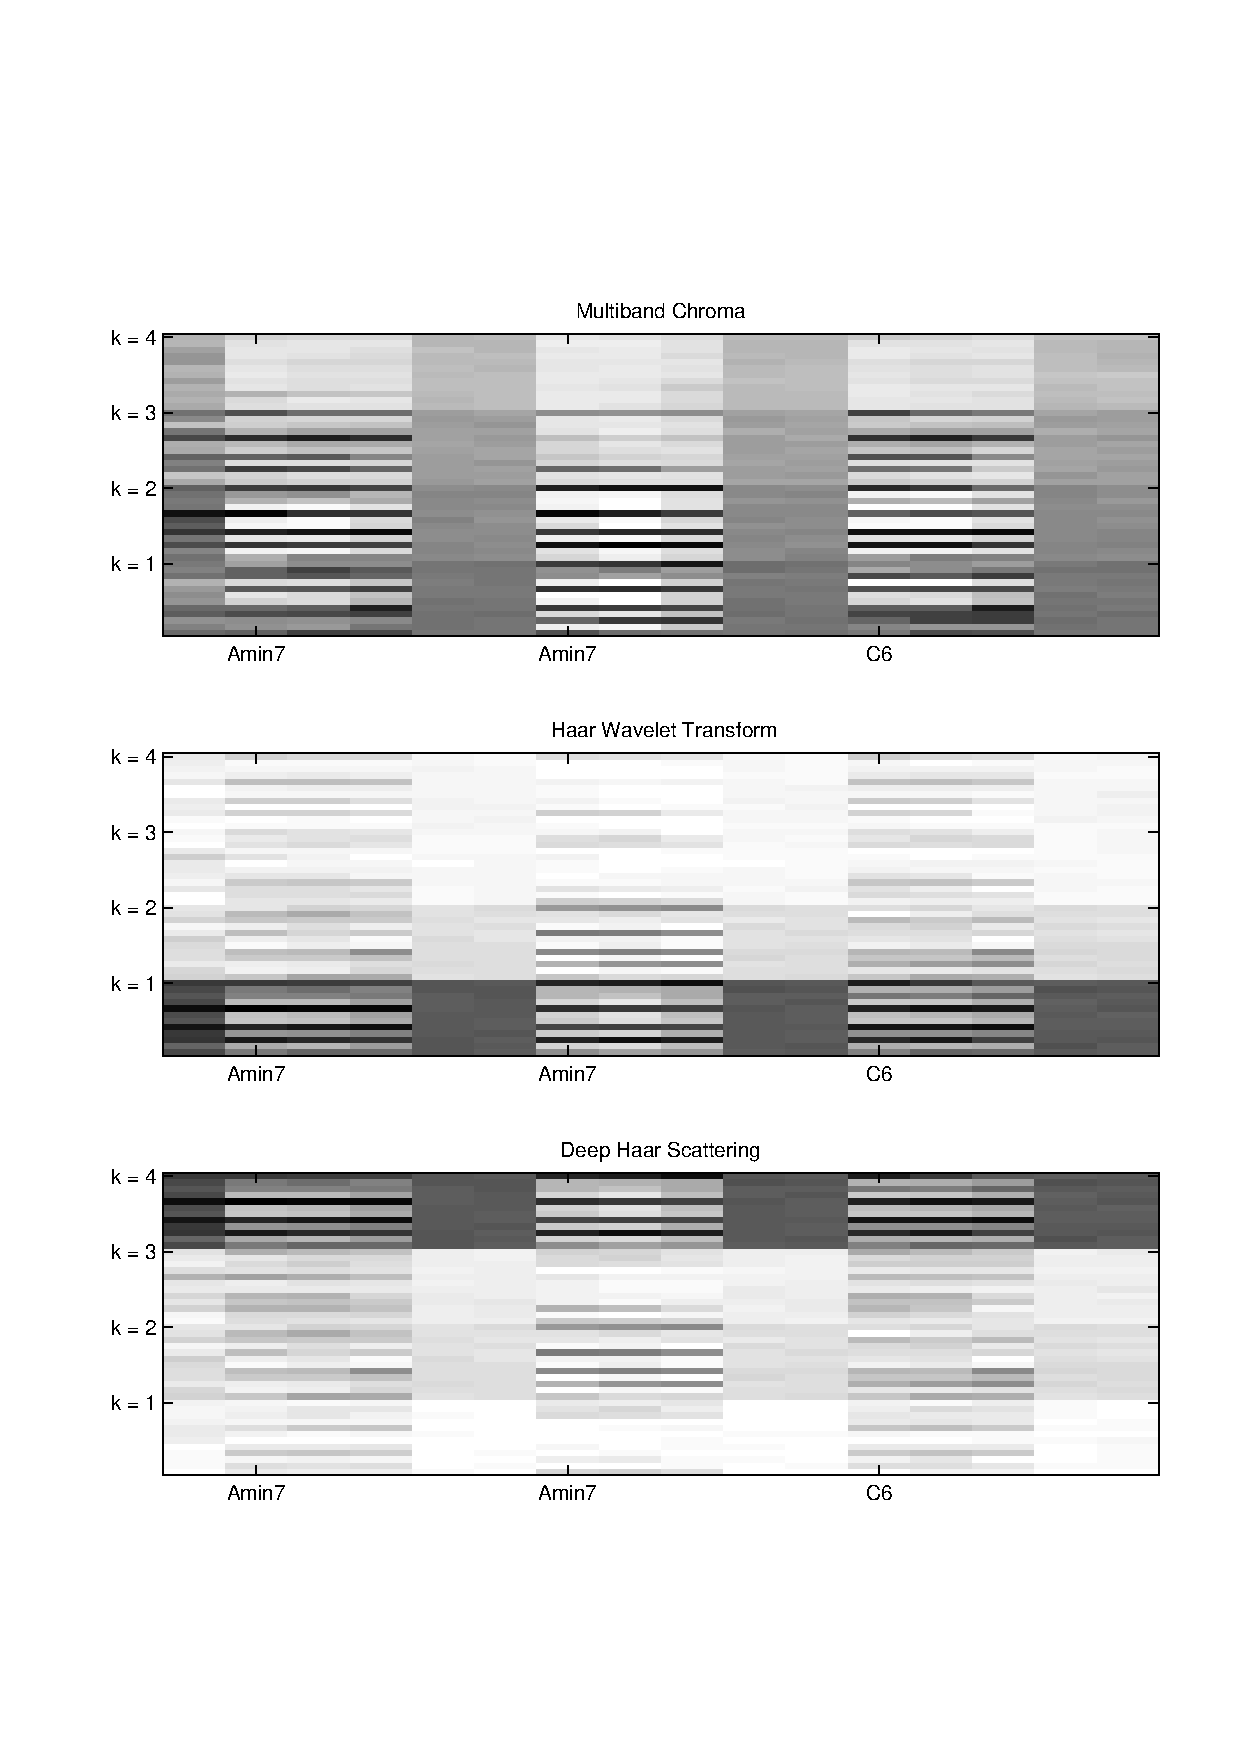
\includegraphics[width=6cm]{figs/features_gray.pdf}
	\end{center}
\caption{Features for chords in Figure 1 for $K=4$: multiband chroma (top), Haar wavelet transform (middle), deep Haar scattering (bottom).}
\label{fig:features}
\end{figure}

\begin{table}
	\begin{center}
	\begin{tabular} {| c | c | r |}
	\hline
	$K$ & Mode & Distance \\
	\hline
	4 & Multiband & 0.5653 \\
	& Wavelet & 0.5920 \\
	& Scattering & 0.5551 \\
	\hline
	8 & Multiband & 0.5937 \\
	& Wavelet & 0.6419 \\
	& Scattering & \textbf{0.6681} \\

	\hline
	\end{tabular}
	\end{center}
	\protect\caption{Ratio between d($\chi_1,\chi_3$) and d($\chi_1,\chi_2$), where the bigger ratio separates $\chi_1$ and $\chi_3$ while bringing $\chi_1$ and $\chi_2$ closer in the feature space for the given feature extraction method and $K$.
	\label{table:distances}}
\end{table}

The example chords in the sequence discussed at the beginning of this paper in Figure \ref{fig:sheet-music} --- Amin7 ($\chi_1$), Amin7 up one octave ($\chi_2$), and C6 ($\chi_3$) --  are played one after another on a piano and analyzed. Figure \ref{fig:features} shows all three features for this isolated chord sequence at $K=4$ for visual simplicity. 

In seeking to separate the feature profile of the C6 chord from the other two, we calculate the Euclidean distance between vectors at temporal frames in the middle of chord activation for each chord. By maximizing the ratio $d(\chi_1,\chi_3)/d(\chi_1,\chi_2)$, the two Amin7 chords are closer in the feature space while the Amin7 and C6 are further.

Table \ref{table:distances} shows these distance ratios for our example chord progression. At scale $K=4$ the wavelet transform wins, while scale $K=8$ provides for higher disambiguation overall, with wavelet scattering separating $\chi_1$ and $\chi_3$ the most, further motivating the use of wavelet transforms for disambiguation of difficult chords with inversions.

%%%%%%%%%%%%%%%%%%%%%%%%%%%%%%%%%%%%%%%%%%%%%%%%%%
\section{Experimental Setup and Evaluation}\label{sec:experiment}

In all experiments, a training set consisting of 108 songs from the Beatles
discography, 99 RWC pop songs, 224 songs from the Billboard dataset, and 20 Queen songs was used for a total of 451 songs.
The testing dataset comprised of 65 songs from the Beatles and uspop datasets that were not part
of the training set and that contained a sufficient number of examples of each chord quality. 
Both the training and testing set of songs are kept constant across all experiments.
	
We consider a large vocabulary of chords with 13 different qualities:
major, minor, minor 7th, dominant 7th, major 7th, suspended 4th, major 6th, minor 6th, suspended 2nd, diminished triad, augmented triad, half-diminished 7th, diminished 7th.
To the list of all possible pairs of chord roots and chord qualities,
we add the null label \texttt{N}, which indicates that no discernible chord is active.
The total number of classes in the extended vocabulary is thus equal to
$12 \times 13 + 1 = 157$.
For each experiment, a chord model and Viterbi transition probability matrix are generated from the  training set with the band $K$ of any experiment determining the amount of chroma vectors at any given temporal window.
$K$ is therefore equivalent to the number of bands in the multiband chroma representation and the maximum wavelet scale ($K = 2^J$) in the wavelet and scattering representations, \ie the number of wavelet coefficients.
Chord recognition is then carried out on a testing set.

After generating estimated chord labels for each song in the test set, Python scripts evaluate the results through the use of the mir\_eval package \cite{raffel2014mir}.
As per \cite{raffel2014mir}, there is ``no single right way to compare two sequences of chord labels,"
and mir\_eval package computes ACE accuracy based along a handful of metrics.
In this experiment we consider two evaluation metrics. The \textbf{mirex} metric ``considers a chord
correct if it shares at least three pitch classes in common" \cite{raffel2014mir}. This metric, however, is too lenient when considering inversions and rarer chord classes (such as min7, maj6). The \textbf{tetrads\_inv} metric is much stricter, evaluating chord accuracy over the entire quality in closed voicing, and taking inversions notated in the reference labeling into account.


	
%%%%%%%%%%%%%%%%%%%%%%%%%%%%%%%%%%%%%%%%%%%%%%%%%%
\section{Results}\label{sec:results}

\begin{figure*}[h!]
\centering
\begin{minipage}{\columnwidth}
	\centering
	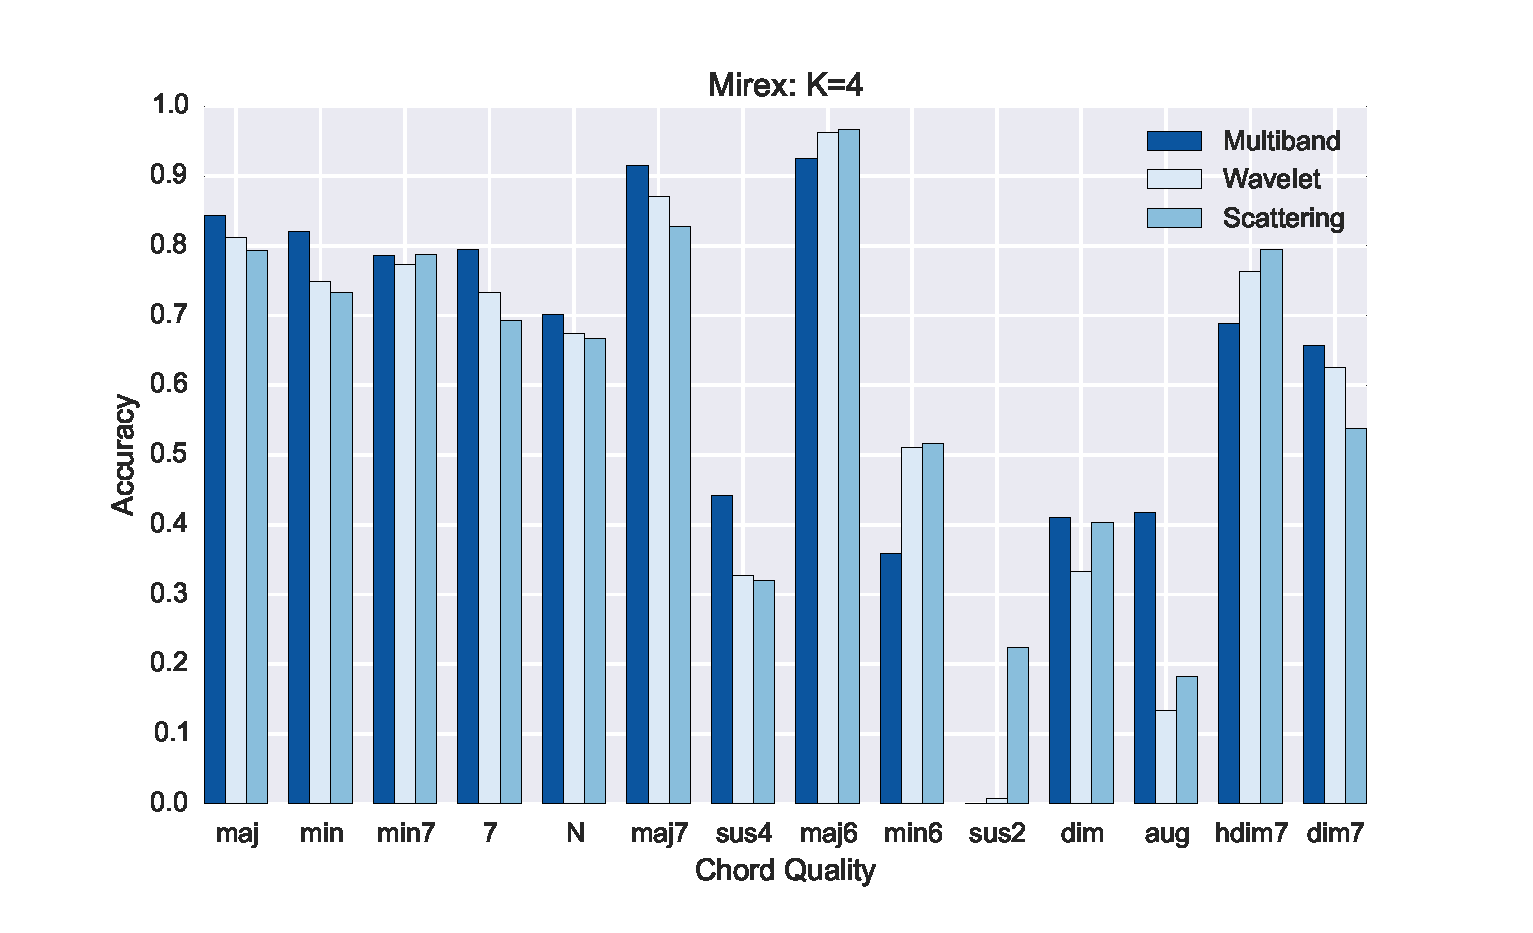
\includegraphics[width=1.05\columnwidth]{figs/mirex4.eps}
\end{minipage}
\begin{minipage}{\columnwidth}
	\centering
	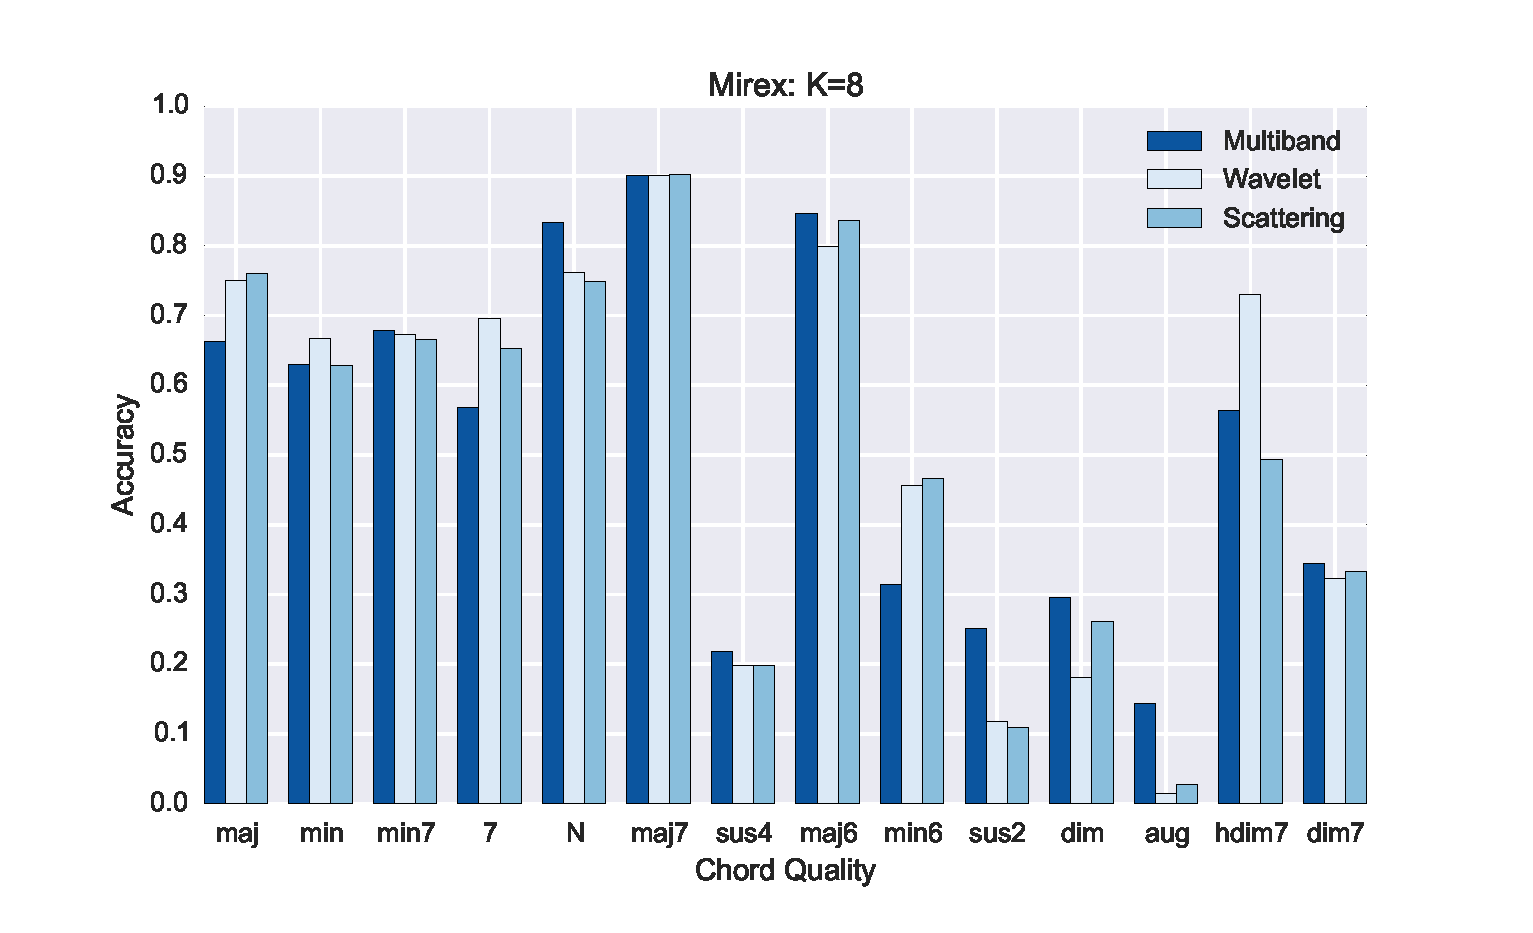
\includegraphics[width=1.05\columnwidth]{figs/mirex8.eps}
\end{minipage}
\caption{Multiband chroma, Haar wavelet transform, and deep Haar scattering compared for $K=4$ (left) and $K=8$ (right) streams. Chord accuracy computed via mirex.}
\label{fig:mirex}
\end{figure*}

\begin{figure*}[h!]
\centering
\begin{minipage}{\columnwidth}
	\centering
	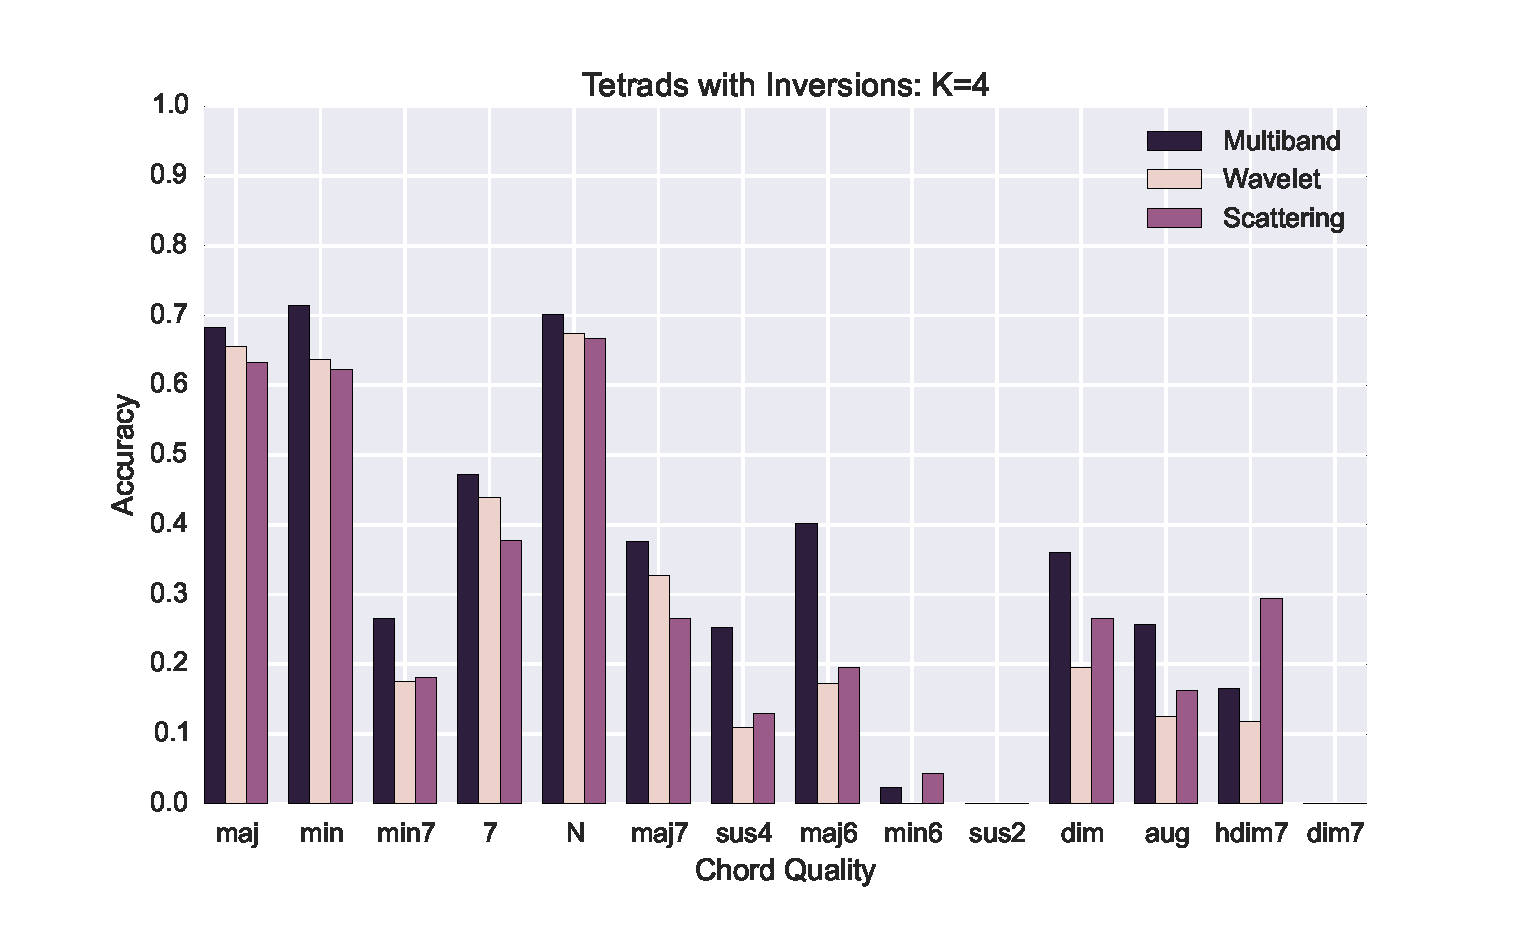
\includegraphics[width=1.05\columnwidth]{figs/tetrad_inv4.eps}
\end{minipage}
\begin{minipage}{\columnwidth}
	\centering
	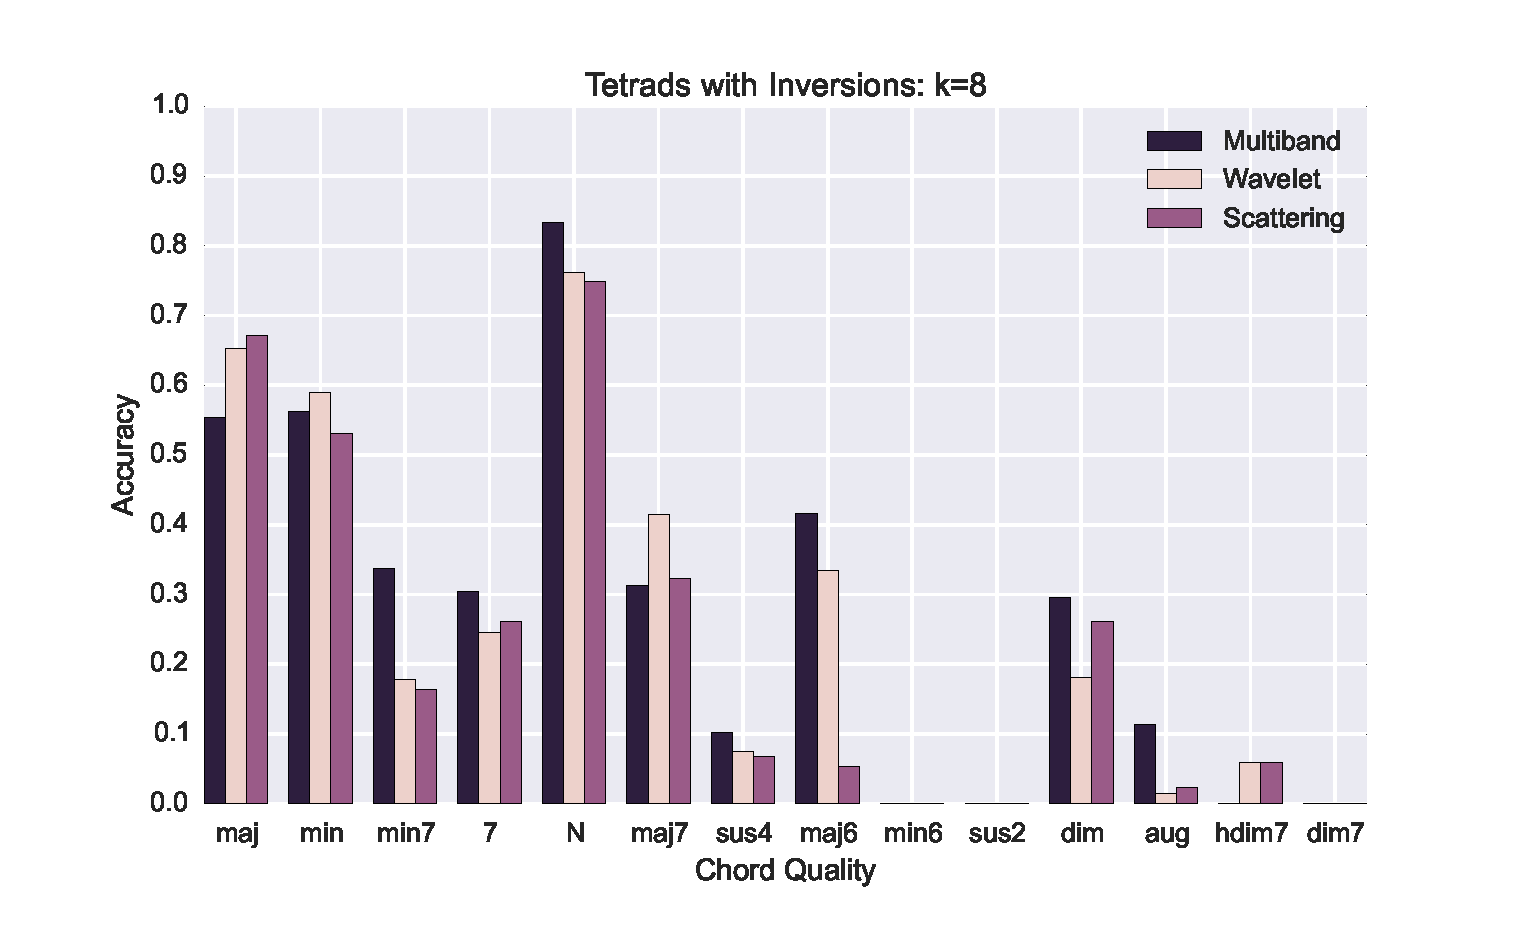
\includegraphics[width=1.05\columnwidth]{figs/tetrad_inv8.eps}
\end{minipage}
\caption{Multiband chroma, Haar wavelet transform, and deep Haar scattering compared for $K=4$ (left) and $K=8$ (right) streams. Chord accuracy computed via tetrads with inversions.}
\label{fig:tetrads}
\end{figure*}

\begin{table}
	\begin{center}
	\begin{tabular} {| c | c | r  | r |}
	\hline
	$K$ & Mode & mirex & tetrads inv \\
	\hline
	4 & Multiband & \textbf{80.18} \% & 62.48 \% \\
	& Haar Wavelet & 75.87 \%  & 58.22 \%\\
	& Haar Scattering & 74.38 \%  & 56.47 \% \\
	\hline
	8 & Multiband & 61.69 \% & 49.18 \% \\
	& Haar Wavelet & 69.36 \% & 55.59 \% \\
	& Haar Scattering & 68.78 \% & 55.44 \% \\
	\hline
	\end{tabular}
	\end{center}
	\protect\caption{Overall accuracy for multiband chroma, Haar wavelet transforms, and deep Haar scattering at scales $K=4$ and $8$. Accuracy computed via mirex and tetrads with inversions metrics.
	\label{table:overall-scores}}
\end{table}

Table \ref{table:overall-scores} shows the accuracy of our automatic chord estimation system for all three feature extraction methods: multiband chroma, Haar wavelet transforms, and deep Haar scattering. Each method is computed at two different scales: $K=4,8$. For multiband chroma, $K$ refers to the number of bands in the representation, where $K=4$ windows the pitch space $\mathbf{X}[t, \gamma]$ with Gaussians covering approximately two octaves. For both wavelet transforms and wavelet scattering, at scale $K=4$, each pitch representation $\mathbf{X}[t,\gamma]$ is reduced to a 4-band multiband chroma representation, and a $J=2=log_2(K)$ wavelet transform/scattering is computed. 

In Table \ref{table:overall-scores} we see that the state-of-the-art $K=4$ multiband results in the best accuracy using both mirex and tetrads with inversions evaluation metrics. At $K=4$ wavelet transforms and scattering suffer by roughly 5\% overall for both mirex and tetrads\_inv. Yet at $K=8$, wavelets and scattering both improve significantly on the multiband representation for both evaluation metrics. While all results for $K=8$ are lower than their partners in $K=4$, the Haar wavelets and Haar scattering representations certainly improve on multiband chroma when treating all octaves independently of each other. In the context of large vocabulary chord estimation, however, the vast majority of chords in our dataset are major, with minor chords more rare, and the rest of our chord qualities even rarer. This heavily skews these overall scores towards accuracy in determining major chords, and therefore a deeper analysis by chord quality is required.

Figure \ref{fig:mirex} shows accuracy by chord quality, filtering all reference labels on the given chord quality, and evaluating chord estimation via mirex. Wavelet transform and scattering improves on some rarer chord qualities for $K=4$ (maj6, min6, sus2, hdim7) and takes modest hits in the more common chord classes. With $K=8$, wavelet transforms and scattering actually improve on major and minor detection, as well as dominant 7th and others. As noted in Section 5, however, the mirex evaluation criteria is rather lenient, so we need to look at the stricter tetrads metric.

In Figure \ref{fig:tetrads} we see accuracy by chord quality computed via tetrads, taking inversions labeled in the reference annotations into account. For $K=4$ bands, our methods do not improve on the multiband chroma, though we see scattering does a bit better for min6 and hdim7 qualities. Increasing scale to $K=8$, however, we see both the wavelet transform and scattering improve detection of major chords, while the wavelet transform provides some slight improvement to minor chords and major 7ths as well. 
	
%%%%%%%%%%%%%%%%%%%%%%%%%%%%%%%%%%%%%%%%%%%%%%%%%%

\section{Discussion and Future Work}\label{sec:conclusion}

Our results do not yet show improved performance of the Haar wavelet transform or scattering over the state-of-the-art multiband chroma approaches for large vocabulary chord recognition, but we do notice that these two wavelet representations code for structures that multiband chroma does not when octaves are treated as independent ($K=8$). Multiband and wavelet analysis differ significantly in that multiband chroma looks at multiple frequency locations while the wavelet representations are multiresolution approaches. Perhaps the question is not whether to use one or the other but when to use both.

There are a few culprits that affect performance of our chord estimation system with the wavelet representations. As seen back in Figure \ref{fig:features} which shows the features for three different chords at $K=4$, we notice that energy is far more spread out among the $K$ chroma streams in the multiband representation as opposed to both the wavelet transform and wavelet scattering. Both concentrate energy much more tightly in certain streams and therefore affect pattern matching downstream as streams with more sparse energy distribution vote less confidently for chord labels in the GMMs. Normalization of each $k$ stream may improve voting accuracy.

Additionally, late fusion of the GMM probabilities plays a central role in our current chord estimation system, as each $k$ stream is treated as independent and then combined after GMM likelihood estimation via geometric mean. Fusion by geometric mean, while sensible for multiband chroma, is more problematic when each stream represents wavelet coefficients of different scales as these streams are not similar to each other. Future work will explore whether fusion by arithmetic mean improves accuracy or whether our GMMs should instead be trained on all $K$ streams together rather than independently. 



% geometric vs. average mean since wavelet bins are not similar (like chroma bins)

% normalize wavelet/scattering coeffs since energy is concentrated at lower scales as compared to multiband, which distributes energy more evenly among bands

% multi resolution representation -- makes sense to classify on K streams together instead of independantly 

%multiband looks at multiple frequency locations while wavelet is a multi resolution approach -- perhaps we should be using them together? the combination could potentially give better results than either individually


%%%%%%%%%%%%%%%%%%%%%%%%%%%%%%%%%%%%%%%%%%%%%%%%%%

% For bibtex users:
\bibliography{WaveletScatteringISMIR2016}
%\bibliographystyle{ieeetr}

% For non bibtex users:
%\begin{thebibliography}{citations}
%
%\bibitem {Author:00}
%E. Author.
%``The Title of the Conference Paper,''
%{\it Proceedings of the International Symposium
%on Music Information Retrieval}, pp.~000--111, 2000.
%
%\bibitem{Someone:10}
%A. Someone, B. Someone, and C. Someone.
%``The Title of the Journal Paper,''
%{\it Journal of New Music Research},
%Vol.~A, No.~B, pp.~111--222, 2010.
%
%\bibitem{Someone:04} X. Someone and Y. Someone. {\it Title of the Book},
%    Editorial Acme, Porto, 2012.
%
%\end{thebibliography}

\end{document}
